% ============================================================
%  Chapter fragment -- included by main.tex
%  (not a standalone document; compile main.tex to build the PDF)
% ============================================================

\sheettitle{09 -- Malware 2: Detection, Evasion \& Anti-Virus}{SWS2 -- ZHAW / Tellenbach}

% ==================== WHY DEFENCE IS WEAK ====================
\section{Why Malware Defence Is Weak \hl{(!)}}
\textit{(LOC = Lines of Code = size/complexity of a program.)}
\begin{itemize}
\item \hl{Can a tool detect 100\% of viruses?} \kw{No} -- in general \kw{undecidable} (like the halting problem). Detection is always an approximation.
\item \kw{LOC asymmetry (attack surface)}: average malware is \kw{tiny} (few k LOC); the things the defender must keep flawless are \kw{huge}. Sizes \kw{relative to average malware}: \kw{120$\times$} Stuxnet, \kw{500$\times$} a text editor, \kw{100{,}000$\times$} an AV tool, \kw{1{,}000{,}000$\times$} the OS. $\Rightarrow$ attacker needs \kw{tiny code to hit one flaw}; defender must secure \kw{millions of LOC} (more code = more bugs). \textit{Silver lining: malware is small $\to$ \kw{analysable}.}
\item \kw{Prospect theory} (\hl{separate, behavioral} reason): \kw{risk-averse for gains, risk-taking for losses} -- prevention is a \kw{certain cost now} for an \kw{uncertain} benefit, so we \kw{gamble} \& act only \kw{after} being hit.
\item Detecting \kw{in-the-wild} malware is "easy" \kw{as long as the characteristics don't change}.
\item \hl{Chicken-and-egg}: to know how to detect malware you must \kw{analyse} it -- but to analyse it you must first \kw{find a sample}.
\end{itemize}

% ==================== DETECTION OVERVIEW ====================
\section{Detection -- Overview \hl{(!)}}
AV uses \kw{multiple engines}, classified by \kw{detection technique} $\times$ \kw{input data} (hybrids common).

{\footnotesize
\setlength{\tabcolsep}{3pt}
\renewcommand{\arraystretch}{1.1}
\arrayrulecolor{zhawblue}
\noindent\begin{tabular}{@{}>{\raggedright\arraybackslash}p{0.30\linewidth}>{\raggedright\arraybackslash}p{0.62\linewidth}@{}}
\rowcolor{zhawblue}
{\color{white}\bfseries Technique} & {\color{white}\bfseries Idea}\\
\rowcolor{tableblue}
Signature & match \kw{known} byte-level characteristics (hash / fuzzy-hash / byte seq)\\
\rowcolor{white}
Heuristic & expert \kw{rules + weights} on file structure / emulated code\\
\rowcolor{tableblue}
Behavior & what the sample \kw{does} (host \& network actions)\\
\rowcolor{white}
Reputation & what's \kw{known} about a file/URL/IP (prevalence, age, origin)\\
\end{tabular}}

\subsection{Input data: Static vs Dynamic}
\begin{itemize}
\item \kw{Static}: data \kw{without executing} -- file metadata (PE header), binary/code, assembly, API/syscalls.
\item \kw{Dynamic}: data \kw{while executing} -- memory, network traffic, filesystem, API/syscalls.
\item Run \kw{natively (with hooking)}, in an \kw{emulator}, or a \kw{VM}. Collecting from a \kw{different layer} (e.g. host watching a VM) $\to$ malware has a \kw{harder time noticing} it's analysed.
\end{itemize}

% ==================== AV ARCHITECTURE ====================
\section{AV System Architecture}
\kw{Host-based} \& \kw{network-based}; most have \kw{client (local)} + \kw{cloud} parts.
\begin{itemize}
\item \kw{Cloud} = "instant update" (signatures hosted there); \kw{local cache} for lost connectivity holds \kw{"most relevant" signatures only}.
\item \kw{Bandwidth}: first send only \kw{metadata} -- file's \kw{(fuzzy) hash/fingerprint}, how it came to be, how it behaved. \kw{Unknown} files $\to$ \kw{quarantine} + send to cloud for analysis.
\item Network: \kw{Content Analysis System} -- \kw{whitelist}$\to$allow, \kw{known malware}$\to$block, \kw{unknown}$\to$send to \kw{sandbox}.
\end{itemize}

\subsection{Layered cloud protection \hl{(!)}}
A \kw{funnel} of layers, \kw{fast/cheap $\to$ slow/expensive}; each filters out most files so only the \kw{truly unknown} fall deeper (you can't sandbox \kw{every} file).
\begin{itemize}
\item \kw{CLIENT}: local-ML / behavior / generics / heuristics -- \kw{ms}.
\item \kw{CLOUD}: metadata-ML (\kw{ms}) $\to$ sample-analysis-ML (\kw{s}) $\to$ \kw{detonation}/sandbox-ML (\kw{min}) $\to$ big-data (\kw{hours}).
\end{itemize}
\hl{Deeper = more victims} (\kw{"block at first sight"}): caught at \kw{ms} $\to$ \kw{0 infected}; only a slower layer catches it $\to$ \kw{patient zero} (first machine) infected while the cloud thinks; \kw{never} caught $\to$ \kw{all victims} infected.
\textit{Key setting -- "time extension for cloud scanning" (e.g. 50s):} how long the client \kw{holds a suspicious file} awaiting the cloud verdict $\to$ longer = \kw{fewer patient-zero} cases but more delay (the "yes*").
\kw{Update feedback}: once a deep layer decides, it \kw{pushes a signature to all clients} $\to$ next time blocked instantly at the ms-layer (one machine's pain = everyone's protection).

\textit{Ex flow (\texttt{invoice.exe}, hold=50s):} 1) \kw{CLIENT} (ms): whitelist/heuristics/local-ML -- unknown $\to$ \kw{hold file}, escalate. 2) \kw{CLOUD metadata} (ms): send hash+origin+reputation -- never seen $\to$ deeper. 3) \kw{CLOUD sample-ML} (s): upload file, still unsure (client \kw{still blocking}). 4) \kw{CLOUD detonation} (min): sandbox sees encryption+C2 $\to$ \hl{malicious} -- but \kw{min $>$ 50s} so the client \kw{already released} it $\to$ \kw{patient zero infected}. 5) \kw{update} pushed to all clients $\to$ everyone after is blocked at ms. \textit{(Bigger hold window $\to$ wait for detonation $\to$ even patient zero saved, but more delay.)}

% ==================== SIGNATURES ====================
\section{Signatures}
Capture \kw{unique characteristics at byte-level}. Types: \kw{hashes}, \kw{fuzzy-hashes}, \kw{byte sequences}. Tens of thousands added \kw{daily}; clever structures check a sample vs all in \kw{$<$30ms}. Backed by \kw{whitelisting} (known-good) + \kw{context} (size, origin).

\subsection{Hashes}
MD5/SHA-1 etc. to check if a file is known \kw{malicious/benign}. \hl{Problem:} \kw{polymorphic/mutating} malware -- \kw{1 changed bit $\to$ totally different hash}. Today mainly a \kw{pre-filter/speedup} (skip re-analysing known files; known files not sent to cloud/sandbox). $\to$ want a signature \kw{robust to modifications}.

\subsection{Fuzzy hashes \hl{(!)}}
\hl{Normal vs fuzzy} -- opposite goal:
\begin{itemize}
\item \kw{Normal hash} (MD5/SHA): \kw{avalanche} -- 1 bit changed $\to$ \kw{totally different} output. Only answers \kw{"exact same file?"} (yes/no), no notion of "close" $\to$ attacker changes 1 byte \& \kw{evades}.
\item \kw{Fuzzy hash}: \kw{similar input $\to$ similar hash} $\to$ gives a \kw{similarity \%} ("86\% like ransomware X") $\to$ survives \kw{polymorphism}, catches whole \kw{families}.
\end{itemize}
\textit{How: normal hash mashes the \kw{whole file} (change spreads everywhere); fuzzy chops into \kw{pieces}, hashes each $\to$ a change only alters \kw{that piece} of the signature.}

Find \kw{similar} files. Byte-by-byte compare (xxd+diff) is accurate but \kw{doesn't scale} 1-to-many $\to$ generate a \kw{fuzzy hash (=signature)} \& compare to stored ones.

\textbf{1st attempt -- fixed 4-byte blocks (fails):} sum each block's ASCII $\to$ mod 64 $\to$ 1 base64 char per block. \kw{Substitution} = 1 char changes (OK), but an \kw{insertion shifts all later blocks} $\to$ every following summary changes $\to$ \hl{looks totally different} though nearly identical.

\textbf{2nd attempt -- CTPH} (Context-Triggered Piecewise Hashing, e.g. \kw{ssdeep}): let the \kw{content} set block boundaries. A \kw{rolling hash} over the \kw{last s bytes} hits a \kw{trigger value} (e.g. \kw{7}) $\to$ marks a \kw{reset point} (boundary); hash each block, combine. ssdeep distance = \kw{edit distance}.
\begin{center}
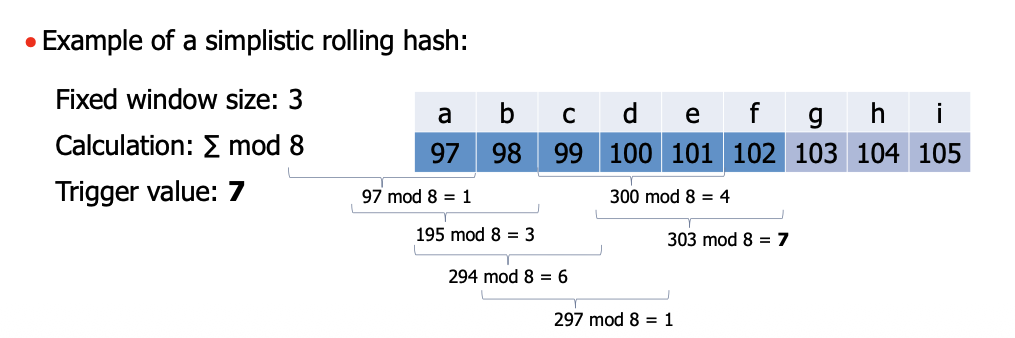
\includegraphics[width=\linewidth]{Figures/rolling_hash.png}
\end{center}
\textit{Insert an \kw{h}: only the \kw{local} block changes, the content-defined boundaries \kw{re-sync} $\to$ rest of the signature stays $\to$ \hl{still similar} (VUUD vs VUH1D).}
\begin{center}
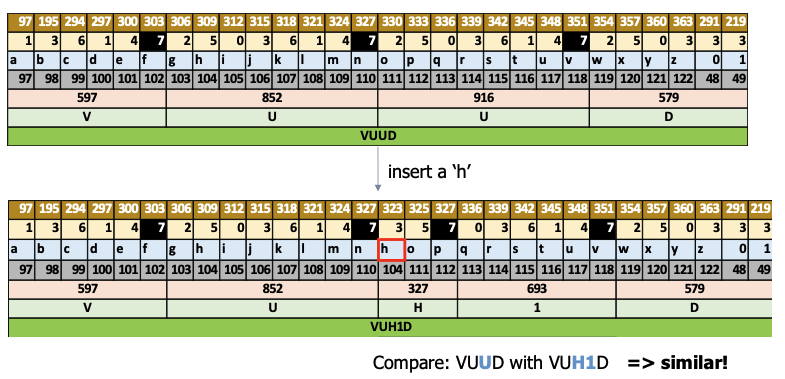
\includegraphics[width=\linewidth]{Figures/table_insert_example.png}
\end{center}
\begin{itemize}
\item \kw{ssdeep blocksize}: depends on file size; two files comparable \kw{only if they share a blocksize} $\to$ files differing $>\sim$3 orders of magnitude \kw{can't be compared}.
\item \kw{sdhash}: statistically \kw{improbable 64-byte} features (Bloom filters) -- good for \kw{partial} matches (copied parts).
\item \kw{tlsh}: \kw{frequency of n-grams} -- good when samples share \kw{building blocks} (reordered code). \hl{Most robust} (ssdeep degrades fastest under nop-insertion).
\end{itemize}

\subsection{Byte sequences \& YARA}
Characteristic byte/string pattern. \kw{YARA} = rule language to \kw{identify \& classify} malware (open-source, multi-platform): \kw{strings} (\texttt{\$a="..."}) + a \kw{condition} (e.g. \texttt{\$mz at 0 and any of \$a*}). Also used for Office-doc analysis (olevba), forensics, IDS.

% ==================== HEURISTICS ====================
\section{Heuristics}
\kw{Rules + weighting} written by \kw{domain experts}.
\begin{itemize}
\item \kw{Static heuristic}: file structure/metadata \& code organization (suspicious sections, \kw{writable code section}, import by ordinal).
\item \kw{Dynamic heuristic}: \kw{emulate} the code to extract features for the rules.
\item Each AV uses \kw{proprietary} algorithms. vs \kw{Behavior}: terms overlap, but heuristics is \kw{more general} (not just behavior) \& runs \kw{before} runtime-behavioral analysis.
\end{itemize}
\textit{Ex: if rule A (RtlMoveMemory...) + B (CreateMutexA "...") + C (GetSystemDirectory) all match $\to$ \kw{PoisonIvy}.}

% ==================== BEHAVIOR ====================
\section{Behavior}
\kw{Semantic} detection -- based on \kw{what the malware does} $\to$ \hl{unaffected by changing the malware's form}. Host \& network often handled by separate engines.
\textit{Monitored:} HOST -- files created/modified, \kw{registry} changes, \kw{processes spawned}; NET -- sockets, connections to specific hosts/domains, \kw{protocol structure} (length/encoding/headers).

\subsection{Sandbox}
Run the sample in a \kw{controlled env} $\to$ study behavior \kw{without affecting other systems}; monitor \kw{syscalls} + network. \kw{Assumption: it behaves as in the wild} (often false -- see evasion). \kw{Cuckoo Sandbox}: Win/OSX/Linux/Android; traces API, dumps+analyses traffic (even \kw{encrypted}), memory analysis (Volatility). Arch: \kw{Cuckoo host} + clean \kw{analysis-VM guests} + isolated virtual network + Internet/\kw{sinkhole}.

% ==================== REPUTATION ====================
\section{Reputation}
Based on what's known about a resource (file/URL/IP):
\begin{itemize}
\item \kw{Prevalence}: used on many machines $\to$ slightly \kw{positive}.
\item \kw{Age}: recently registered/unknown $\to$ neutral/\kw{negative}.
\item \kw{Origin}: downloaded from Internet \& to be executed $\to$ \kw{negative}.
\item Prevalence + Age (widely used \& $>$1 year old) $\to$ \kw{positive}.
\end{itemize}
\hl{Malware dilemma:} \kw{mutate more} $\to$ low prevalence/bad reputation $\to$ suspicious; \kw{mutate less} $\to$ easy \kw{signature} detection.

% ==================== ML ====================
\section{AV \& Machine Learning}
Next-gen "signatures": signatures/heuristics/behavior are \kw{learned}, not hand-crafted. \kw{Train a model} on millions of data points from \kw{static} (file attributes -- \# sections, is DLL/EXE, has debug info...) or \kw{dynamic} (behavior) analysis. Static = examine attributes \kw{without running} (Cylance pioneered). Active research field.

% ==================== EVASION ====================
\section{Evasion \hl{(!)}}
\textit{Each technique counters a specific detection type.}

\subsection{Generic}

For example to avoid detection, one needs to rename his malware (.exe) files will most likely be blocked by emails etc.

\begin{itemize}
\item \kw{File formats}: \kw{rename} \texttt{.exe}$\to$\texttt{.hex} (circumvent extension \kw{blacklists}; needs social-eng to rename back). AV must parse \kw{many formats} (PDF, GIF) $\to$ \kw{decoder vulnerabilities} = attack vector (McAfee disabled by a crafted file, 2016). Many Win executable formats (\kw{lnk, pif, wsh}); .lnk can link to \kw{cmd.exe /C}.
\item \kw{Compression}: compressed files are normal \& must be \kw{decompressed} (slow) $\to$ gateways may \kw{skip} it (large/nested \kw{ZIP-bomb} DoS/high-load) $\Rightarrow$ default = detect+block. \kw{Password-protected/encrypted} archives: AV \kw{can't inspect}, but denying isn't an option (legit use).
\end{itemize}

\subsection{Signature evasion: Polymorphism}
\kw{Polymorphic engine} mutates the code while \kw{keeping its function (semantics)} the same. Bundled (self-propagating) or applied \kw{before distribution}. Via \kw{packers/cryptors} = \kw{encrypted payload} + \kw{unpacking/decryption stub}. AV signs the \kw{stub} $\to$ attacker \kw{mutates the stub} (junk instructions, instruction substitution).

\subsection{Heuristic/behavior evasion: Metamorphism}
Like polymorphism but the \kw{whole binary -- incl. the engine itself -- changes}. Idea: translate own code to an \kw{intermediate language}, edit, translate back to machine code. \textit{(Hiding code via packing beats \kw{static} heuristic; beating \kw{dynamic} heuristic needs the emulator to fail to unpack.)}

\subsection{Sandbox / emulation evasion}
\begin{itemize}
\item \kw{Fingerprint the environment}: scan for VM/sandbox \kw{registry, hardware, software (VMware Tools), processes} $\to$ \kw{behave benignly} if analysed. (Counter: \kw{custom} virtualization / alter the footprint.)
\item \kw{Human interaction}: wait for \kw{mouse clicks} / dialog responses (CAPTCHA-like) before running the malicious part $\to$ "is this a \kw{real user}?" (arms race: detect vs emulate a human).
\item \kw{Time}: \kw{time triggers} (run only on a date) or \kw{extended sleep} to \kw{outwait} the sandbox (counter: sandbox shortens sleep / extends analysis).
\end{itemize}
\textit{Combining multiple free packers can bypass many AV engines at once.}

% ==================== HOW GOOD ====================
\section{How Good Is Anti-Virus?}
\begin{itemize}
\item Hard to assess: next-gen vendors push \kw{own tests}; \kw{independent} tests (AV-Test, AV-Comparatives, MRG Effitas, per \kw{AMTSO}) exist but are often \kw{vendor-sponsored}; results depend on \kw{methodology \& sample set}.
\item \kw{Retrospective test} (detection with \kw{signatures frozen}, heuristics/behavior offline) shows \kw{proactive} rates $\sim$47--99\%. \textit{Why rarely possible now? modern AV is \kw{cloud-connected} -- you can't freeze it offline.}
\end{itemize}

\begin{defbox}
\textbf{Take-away:} \hl{No AV gives full protection.} Detection = signature / heuristic / behavior / reputation (+ML), over static/dynamic input. Each is countered by an evasion (polymorphism vs signatures, metamorphism vs heuristics, sandbox-fingerprinting vs behavior). If AV is your \kw{only} defence, you \kw{will} likely get infected.
\end{defbox}

